\section{Method: From Two Fixes to a Predictive Distribution}
\label{sec:method}

\begin{figure}[htbp]
  \centering
  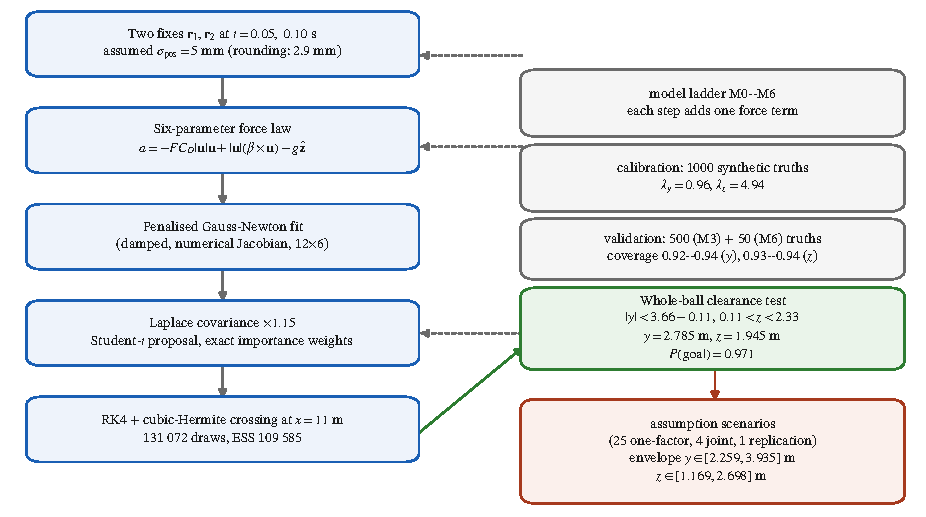
\includegraphics[width=0.83\textwidth]{f17-workflow.pdf}
  \caption{The prediction pipeline of Sections~\ref{sec:model}--\ref{sec:results},
  from the two fixes to the reported interval and probability. Each stage is
  checked against an independent calculation: the integrator against DOP853,
  the Laplace covariance against a second sampler, and the whole chain against
  $750$ synthetic truths: $500$ on M3, $50$ on M6 and $25$ under a law containing
  an extra vertical force.}
  \label{fig:workflow}
\end{figure}

\subsection{The inverse problem and the noise model}

The data are the six coordinates of $\vect r_1$ and $\vect r_2$. The forward map
$\vect F(\vect\theta)=(\vect r(t_1;\vect\theta),\vect r(t_2;\vect\theta))$ carries
the six parameters of Eq.~\eqref{eq:theta} to the two predicted positions, and
the inverse problem is to characterise the set of $\vect\theta$ consistent with
the data. A point inversion is inappropriate for two reasons. The map is
nonlinear, so even with as many data as parameters the solution need not be
unique; and the model is incomplete, because a non-spinning ball can curve
through wake asymmetry \citep{texier2016} and the effective force may vary from
ball to ball. The fitted $\vect\beta$ is therefore an effective coefficient, not
a spin measurement. The same inverse problem has been solved for baseball from a large set of
tracked pitches, where the data could separate drag, lift, and the spin vector
\citep{nathan2008pitchfx}; two fixes cannot support that separation, and the
prior must carry part of the inference. Estimates of
aerodynamic coefficients from a trajectory are also known to depend on the
estimator \citep{jsme2014}, and different conventions for reconstructing spin
give different answers \citep{shorter2013}; a probabilistic treatment makes that
dependence explicit instead of hiding it.

We adopt the measurement model
\begin{equation}
  \vect r_i^{\rm obs}=\vect r(t_i;\vect\theta)+\vect\varepsilon_i,
  \qquad
  \vect\varepsilon_i\sim\mathcal N(\vect 0,\sigma_{\rm pos}^2\vect I_3),
  \label{eq:noise}
\end{equation}
in which each coordinate is observed with independent Gaussian error of standard
deviation $\sigma_{\rm pos}=5$ mm. This value is half of the last printed digit
of the given coordinates, which are quoted to $1$ cm; it is a statement about the
printed data, not a calibration of any tracking system, and the problem supplies
no measurement error. Goal-line technology is certified to about $1.5$ cm
\citep{fifa2020glt}, optical systems in two dimensions only
\citep{fifa2025epts}, and a three-dimensional fix normally requires several
calibrated views \citep{hawkeye_glt}; single-camera reconstruction remains a
research problem \citep{vorobev2025}. The assumed $5$ mm is therefore
optimistic, and \S\ref{sec:scenarios} repeats the inference with
$\sigma_{\rm pos}$ between $2.5$ and $20$ mm.

Equation~\eqref{eq:noise} treats the two fixes as independent and attributes all
of the error to the position. A real tracking system also stumbles over the
time stamps, and a time error of $\sigma_t$ displaces the measurement along the
flight by $\sigma_t|\vect v|$, which for $\sigma_t=\SI{1}{ms}$ and
$|\vect v|\approx\SI{31}{m\,s^{-1}}$ is already \SI{31}{mm}, six times the
assumed positional error. The natural extension is therefore a block-diagonal
observation covariance,
\begin{equation}
  \vect C_i=\sigma_{\rm pos}^2\vect I_3+\sigma_t^2\,\vect v_i\vect v_i^{\top},
  \qquad i=1,2,
  \label{eq:cov}
\end{equation}
in which the second term is the first-order propagation of a time-stamp error
through the velocity, so that the measurement uncertainty is anisotropic: it is
largest exactly along the direction in which the two fixes carry most of their
information. A common-mode offset, which is the other error mode of a
multi-camera system, is represented by adding
$\sigma_b^2\vect 1\vect 1^{\top}$ to both blocks. Both extensions leave the
likelihood Gaussian and cost nothing numerically; \S\ref{sec:validation}
reports how much they move the prediction, and the answer that we quote is the
one obtained with the isotropic model of Eq.~\eqref{eq:noise}, because the
problem supplies no timing or correlation information and the extensions serve
as a robustness check rather than as a different measurement model.

\subsection{Information content of six coordinates}
\label{sec:audit}

Before fitting, we ask which combinations of parameters the data constrain.
Consider the seven-parameter model in which $\vect\beta$ is a free vector. Its
data Jacobian $\vect J=\partial\vect F/\partial\vect\theta_7$, with every row
divided by $\sigma_{\rm pos}$, is $6\times7$ and has rank $6$: the observations
are blind to one direction in parameter space. The six nonzero singular values
are $327.227$, $318.306$, $217.813$, $1.766$, $1.765$, and $1.750$. The three
large values describe the launch geometry; the three values near $1.75$ describe
the aerodynamic coefficients and are almost degenerate. The blind direction is
dominated by a joint change of the components of $\vect\beta$ and contains the
component along the instantaneous air velocity: when $\vect\beta\parallel\vect u$
the force $|\vect u|(\vect\beta\times\vect u)$ vanishes, so that component
produces no acceleration at first order and the data cannot see it. In the
seven-parameter posterior the variance of this component shrinks by only
$8.69\%$ relative to the prior, against $69.99\%$ and $72.65\%$ for the two
transverse components; a local information count gives about $5.27$
data-determined parameters. This is the concrete form of a sloppy model
\citep{gutenkunst2007}: a spectrum spanning two orders of magnitude, with the
flat directions fixed not by data but by the prior \citep{white2017}.

The six-parameter model of Eq.~\eqref{eq:theta} removes the blind direction by
construction: it sets the along-flight component to zero and fits the two
components that produce a force. This is the largest model the data can support,
and its posterior is conditional on that choice. The cost of the choice can be
measured. In the seven-parameter parameterisation, fixing the lab-frame
component closest to the flight direction and scanning it over $\pm0.075$
m$^{-1}$, with the remaining components refitted at each point, moves the
predicted crossing from $y=2.555$ m to $2.782$ m and from $z=2.116$ m to
$1.849$ m. The changes, $0.228$ m in $y$ and $0.267$ m in $z$, are comparable to
the predictive standard deviation and far larger than the precision of the
fixes. The seven-parameter model is rank-deficient: six observations cannot
identify seven parameters, and its posterior is a conditional statement, not a
measurement. We therefore report the six-parameter posterior and pair it with a
model envelope rather than a single interval.

\subsection{Likelihood and priors}
\label{sec:priors}

With the noise model of Eq.~\eqref{eq:noise}, the likelihood is
\begin{equation}
  p(\vect r_1,\vect r_2\mid\vect\theta)
  \propto\exp\left[-\frac{1}{2\sigma_{\rm pos}^2}
  \sum_{i=1}^{2}\left\|\vect r(t_i;\vect\theta)-\vect r_i\right\|^2\right],
  \label{eq:like}
\end{equation}
with the priors taken as independent normals,
\[
  \vect v_0\sim\mathcal N\!\big((30,0,7),\operatorname{diag}(15^2,15^2,10^2)\big),\quad
  C_D\sim\mathcal N(0.25,0.15^2),\quad
  \beta_i\sim\mathcal N(0,0.008^2),
\]
in which $\vect v_0$ is in \si{m\,s^{-1}} and $\beta_i$ in \si{m^{-1}}; both are
truncated by the hard bounds
\[
  5<v_{0x}<60, \quad |v_{0y}|<30, \quad 0<v_{0z}<30, \quad
  0<C_D<1, \quad |\beta_i|<0.08 ,
\]
in SI units, listed in Table~\ref{tab:priors}. The launch prior is broad compared
with the precision of the fixes, so the data, not the prior, fix the launch
direction. The drag prior is wider than the
wind-tunnel range $0.17$--$0.22$ \citep{carre2005,goff2012}, because the
effective drag of a spinning ball need not match the tabulated value. The transverse prior is centred at zero: it expresses no
preference for left or right curl and no assumption that the force is Magnus.
Its scale, $0.008$ m$^{-1}$, corresponds through
$C_L=|\vect\beta|/\mathrm{FACTOR}$ to lift coefficients of the measured order, so
it admits the observed forces while remaining weak along the two determined
directions. A prior on the spin would instead introduce a particular force law
that the data cannot test \citep{texier2016}; parametrising the force directly is
the more honest choice.

\begin{table}[t]
  \centering
  \caption{Priors and hard bounds on the six parameters. The priors are
  independent normals and the bounds truncate them.}
  \label{tab:priors}
  \begin{tabular}{@{}lll@{}}
    \toprule
    Parameter & Prior & Hard bounds \\
    \midrule
    $v_{0x}$ & $\mathcal N(30,\,15^2)$ m/s & $5$--$60$ m/s \\
    $v_{0y}$ & $\mathcal N(0,\,15^2)$ m/s & $-30$--$30$ m/s \\
    $v_{0z}$ & $\mathcal N(7,\,10^2)$ m/s & $0$--$30$ m/s \\
    $C_D$ & $\mathcal N(0.25,\,0.15^2)$ & $0$--$1$ \\
    $\beta_1$ & $\mathcal N(0,\,0.008^2)$ m$^{-1}$ & $\pm0.08$ m$^{-1}$ \\
    $\beta_2$ & $\mathcal N(0,\,0.008^2)$ m$^{-1}$ & $\pm0.08$ m$^{-1}$ \\
    \bottomrule
  \end{tabular}
\end{table}

\subsection{Posterior computation}
\label{sec:sampling}

We combine likelihood and priors with Bayes' rule and compute the posterior in
two stages: a Laplace approximation locates and scales the target, and exact
importance sampling corrects it. The joint residual is
\begin{equation}
  \vect R(\vect\theta)=\left(
  \frac{\vect r(t_1;\vect\theta)-\vect r_1}{\sigma_{\rm pos}},\,
  \frac{\vect r(t_2;\vect\theta)-\vect r_2}{\sigma_{\rm pos}},\,
  \frac{\vect\theta-\vect\mu}{\vect s}\right),
  \label{eq:residual}
\end{equation}
a vector of length twelve whose first six entries are the data residuals and
whose last six are the prior pulls, with $\vect\mu$ and $\vect s$ the prior
means and standard deviations. The MAP estimate minimises
$\tfrac12\|\vect R\|^2$ under the hard bounds by a damped Gauss--Newton iteration
with a finite-difference Jacobian and adaptive damping, so no derivative of the
integrator is required. The solution has $C_D=0.3466$,
$|\vect\beta|=0.008426$ m$^{-1}$ (equivalently $C_L=0.159$), and crosses the
plane at $y=2.7830$ m, $z=1.9451$ m, $t=0.3988$ s. At the mode, the
Gauss--Newton approximation to the inverse Hessian of $\tfrac12\|\vect R\|^2$
gives the Laplace covariance
\begin{equation}
  \vect C=1.15\left(\vect J^{\mathsf T}\vect J\right)^{-1},
  \label{eq:laplace}
\end{equation}
where $\vect J$ is the $12\times6$ Jacobian of $\vect R$ at the MAP and the
factor $1.15$ inflates the local quadratic approximation.

The Laplace covariance is not a profile-likelihood interval: it is symmetric by
construction and uses the curvature at the mode, whereas a profile interval
follows the likelihood along one parameter after maximising over the others, can
be asymmetric, and along the ridge of \S\ref{sec:audit} can differ
substantially. We therefore use the Laplace covariance only as a proposal. Draws are taken from a multivariate Student-$t$ distribution with
eight degrees of freedom, centred at the MAP with scale matrix $\vect C$; the
heavy tails ensure that the proposal does not underestimate the tails of the
target. Each draw $\vect\theta_j$ carries the exact importance weight
\begin{equation}
  w_j\propto\frac{p(\vect r_1,\vect r_2\mid\vect\theta_j)\,p(\vect\theta_j)}
  {q(\vect\theta_j)},
  \label{eq:weights}
\end{equation}
where $q$ is the proposal density. Because the weights are exact, the weighted
draws represent the posterior itself, not its Laplace approximation, and the
reported intervals are weighted quantiles. We draw $131072$ samples and retain
an effective sample size of $109585$, a ratio that indicates the proposal is
close to the target. A Markov chain would also sample the posterior, but it
would require convergence diagnosis along a ridge and a separate run for every
scenario; independent weighted draws make the twenty-six cases of
\S\ref{sec:scenarios} directly comparable.

The computation was cross-checked: an independent parameterisation of the
transverse force (three lab-frame components instead of two transverse ones), an
independent sampler of $40000$ draws, and an independent reference run of
$131072$ draws all reproduce the prediction; an adaptive DOP853 integration
agrees with the RK4 crossing to better than $2\times10^{-6}$ m; and the
posterior mean, $(2.7847,1.9452)$ m, differs from the MAP by $1.4$ mm in $y$
and $1.0$ mm in $z$.

\subsection{Prediction and goal probability}
\label{sec:prediction}
\label{sec:answer}

Every weighted draw is propagated through the full nonlinear equations to
$x=x_g$ with the RK4 scheme and crossing rule of \S\ref{sec:model}; the map from
parameters to entry point is never linearised. This matters because impact-point
distributions can be markedly non-Gaussian when the entry state and the
aerodynamic parameters are uncertain \citep{williamson2017}, and because
propagating uncertain aerodynamic coefficients to impact dispersion is the
standard use of such fits \citep{mehta2015}. The predictive distribution has
mean $y=2.7847$ m with $90\%$ interval $[2.45,3.12]$ m, mean $z=1.9452$ m with
$90\%$ interval $[1.62,2.27]$ m, and mean crossing time $0.399$ s. A negligible
fraction of the draws does not reach the plane and is excluded, so the
distribution is conditional on reaching it.

A goal is decided for the whole ball by Eq.~\eqref{eq:clearance}: the crossing
is successful if the disc of radius $R$ lies inside the aperture. The goal
probability is the weighted fraction of draws satisfying this criterion,
\begin{equation}
  P(\text{goal})=0.971\pm0.001,
  \label{eq:pgoal}
\end{equation}
where the quoted uncertainty is the Monte Carlo standard error of the weighted
estimate; it measures sampling error, not model error. The assumption-driven
uncertainty is quantified separately in \S\ref{sec:scenarios}.

\subsection{Assumption scenarios}
\label{sec:scenarios}

To measure how much the answer depends on assumptions that two fixes cannot
test, the entire inference --- refit, importance weights, and propagation --- is
repeated under twenty-five single-factor variants of the nominal assumptions,
under four joint-stress combinations, and in one independent replication. The variants are:
$\sigma_{\rm pos}=2.5$, $10$, and $20$ mm; a correlation of $-0.5$ or $0.7$
between the errors of the same coordinate at the two epochs; an epoch jitter of
$0.5$ or $2$ ms, propagated as a position uncertainty along the instantaneous
velocity; a transverse prior width multiplied by $0.5$ or $2$; the prior mean of
$\beta_1$ or $\beta_2$ shifted by one standard deviation in either direction; a
drag prior mean of $0.1$ or $0.4$; a uniform wind of $3$ m s$^{-1}$ along each
axis in both directions; a transverse force with a component along the launch
direction, $\gamma=\pm0.016$ m$^{-1}$; and a drag coefficient with a strong
linear dependence on speed, of either sign.

Across these cases the goal probability ranges from $0.735$ at
$\sigma_{\rm pos}=20$ mm to $0.9997$ at $2.5$ mm, the scenario means from
$2.687$ to $3.130$ m in $y$ and $1.846$ to $2.042$ m in $z$, and the union of
the $95\%$ marginal intervals is $[2.259,3.935]$ m in $y$ and $[1.169,2.698]$ m
in $z$. Four additional joint-stress cases, which combine several adverse
variants, give goal probabilities from $0.561$ to $0.987$ and means from
$2.733$ to $3.339$ m in $y$. A uniform wind is nearly a Galilean
shift of the launch velocity over the short baseline, so the
refit absorbs most of it and a $3$ m s$^{-1}$ crosswind moves the entry by only
$0.007$ m. The two extremes of the goal probability are produced by the fix
precision, not by the aerodynamic model.

This is a discrete scenario envelope, not a confidence or credible interval. The
cases are selected rather than sampled from a distribution over assumptions,
they are not equally probable, and the envelope is not a guaranteed bound. It
answers a narrower question: how far can the prediction move when one assumption
at a time is changed by an amount that a careful analyst might defend? The full
set is reported in \S\ref{sec:results}.

\subsection{Control estimators}

The same six numbers were analysed earlier with two simpler estimators: a
constant-acceleration inversion that fits the two fixes exactly, and a
drag-plus-Magnus Bayesian fit whose spin prior came from the literature. Both
are retained as controls and quantified in \S\ref{sec:results}; neither is used
for the headline prediction.
